\label{sec:coverage_frameworks}

\subsubsection{Ruby test coverage}
There are multiple different ways of analyzing test coverage, and the
properties and conditions for each different kind of test coverage are
discoursed in \fref{sec:coverage}. However, we were unable to find any
test coverage tools for Ruby which analyzed anything else than statement
coverage, which is the weakest test coverage metric. Quite much effort
was spent on finding such tool, but without any success. Several
websites and Stack Overflow-answers indicate that no such tool exists
for Ruby at the time of this writing \cite{web:coverage_ruby19,
so:c1c2_coverage, so:c1_coverage, web:toolbox_code_metrics}.\\

We ended up using the
SimpleCov\footnote{\url{https://github.com/colszowka/simplecov}} tool
for Ruby test coverage metrics. At the time of this writing, it is the
most used Ruby tool for test coverage. It is also actively developed,
works with recent Ruby versions and RSpec versions, and produces pretty
and easy- to-read coverage reports in HTML (see
\fref{fig:simplecov_report}). \cite{web:toolbox_code_metrics}\\

\begin{figure}
\centering
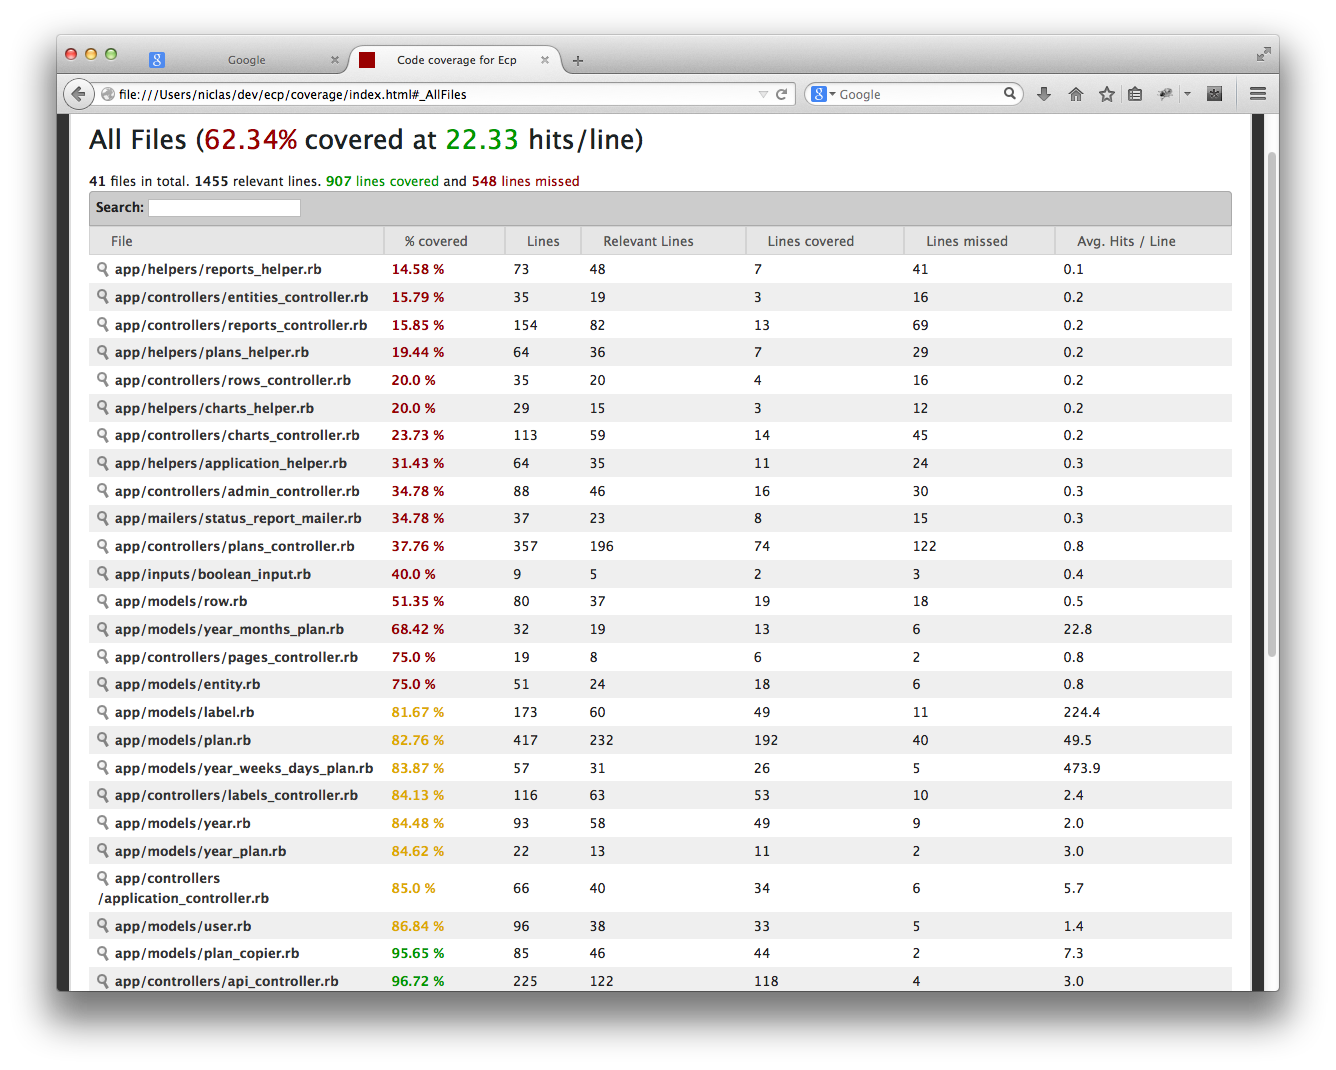
\includegraphics[width=0.8\textwidth]{results/choices/simplecov}
\caption{A test coverage report generated by SimpleCov.}
\label{fig:simplecov_report}
\end{figure}


\subsubsection{CoffeeScript test coverage}
For the client-side CoffeeScript, we used a plug-in for the Karma test
runner called karma-coverage\footnote{\url{https://github.com/karma-
runner/karma-coverage}}. This tool basically integrates Karma with
Ibrik\footnote{\url{https://github.com/Constellation/ibrik}}, which is a
tool developed by Yahoo! for measuring test coverage of CoffeeScript
code. We did initially have some problems with getting this tool to work
correctly, since Ibrik internally uses another CoffeeScript compiler;
CoffeeScriptRedux, than the compiler used when tests itself are run.
CoffeeScriptRedux is more strict and yielded syntax errors in some of
our files that could be compiled correctly in the production code. The
latest available release of Ibrik (version 1.1.1) also had major issues
with certain constructs in CoffeeScript, which made the files impossible
to analyze. These issues were however fixed in the development version.
Ibrik was first released in December 2013, which may explain its
immaturity. Ibrik internally uses istanbul-js for the coverage
analysis and report generation.\\

The chosen solution worked very well after sorting out the issues.
Statement coverage as well as branch coverage is supported, and it
generates useful reports. As with SimpleCov, the coverage reports are
produced as an interactive HTML report (see \fref{fig:karma_report}).\\

\begin{figure}
\centering
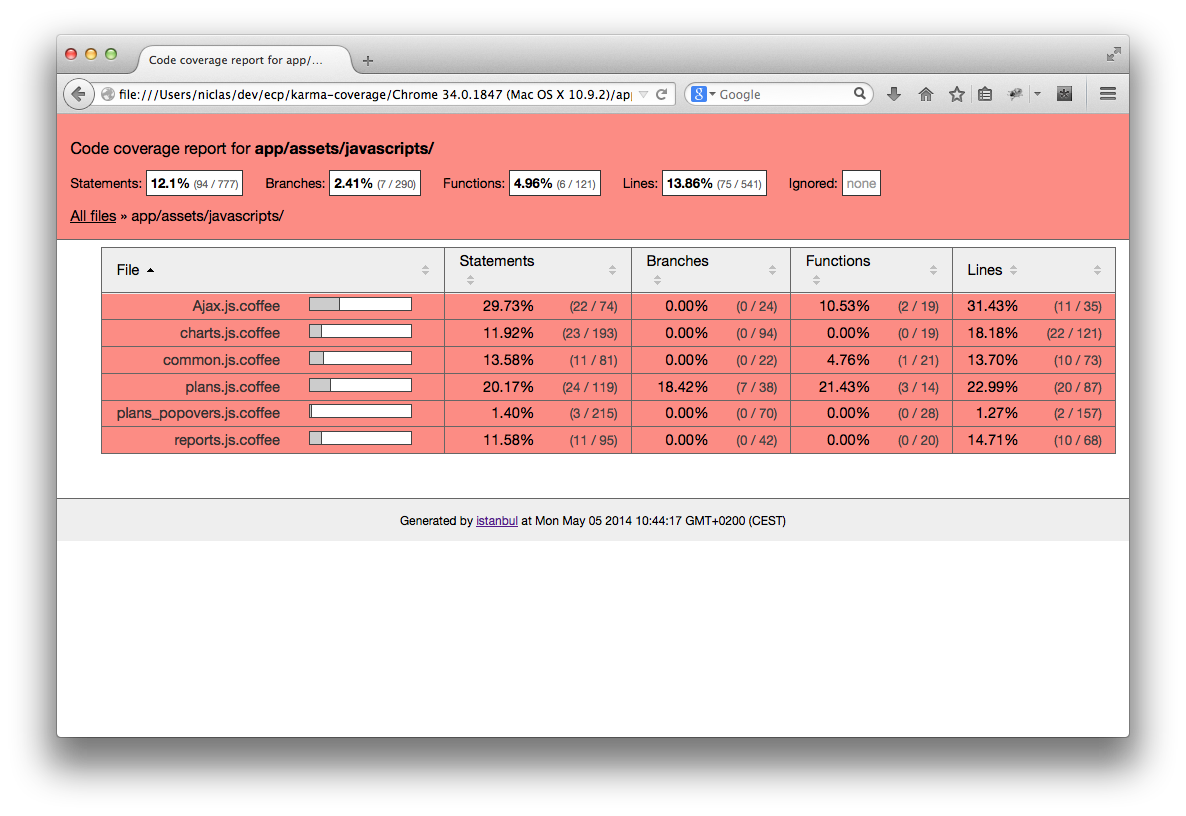
\includegraphics[width=0.8\textwidth]{results/choices/karma_coverage}
\caption{A test coverage report generated by istanbul-js using karma-coverage.}
\label{fig:karma_report}
\end{figure}


\subsubsection{Test coverage issues}

One issue with using test coverage in this particular project is the
fact that very few files were added. Most of the changes were made in
existing classes and files, either as new functions or as changes to
existing functions. Since the overall test coverage is measured per
file, it is impossible to get an exact measure of how well tested the
new and refactored code is, since old and completely untested code
lower the test coverage.\\

We have tried to mitigate this by looking at the coverage reports by
hand, and try to determine a subjective measure of how good the test
coverage is for new and refactored code. \Fref{fig:coverage_example}
shows an excerpt of a coverage report. In this case, our subjective
measure would say that the function |exports.getProduction()| is
completely untested. The function |exports.getLabelId()| is well tested
and has full statement- as well as branch coverage. The function
|exports.formatValues()| has full statement coverage, but non-optimal
branch coverage since the cases where |x| or |y| is not set are not
covered.\\

\begin{figure}
\centering
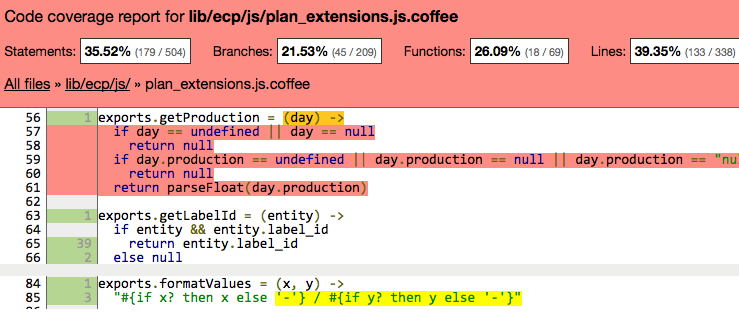
\includegraphics[width=0.8\textwidth]{results/choices/js_coverage}
\caption{An excerpt from a coverage report generated using karma-coverage
         which demonstrates three different types of tested functions.}
\label{fig:coverage_example}
\end{figure}
